\documentclass[UTF8,a4paper,12pt]{ctexart}

\usepackage[margin=1in]{geometry}
\usepackage{setspace}
\usepackage{graphicx}
\usepackage{booktabs}
\usepackage{array}
\usepackage{longtable}
\usepackage{float}
\usepackage{enumitem}
\usepackage{amsmath,amssymb}
\usepackage{hyperref}
\usepackage{xcolor}
\usepackage{tikz}
\usepackage{pgfplots}
\usepackage{caption}

\pgfplotsset{compat=1.18}
\usetikzlibrary{arrows.meta,positioning,shapes.geometric,shapes.misc,fit,backgrounds,calc}

\hypersetup{
  colorlinks=true,
  linkcolor=blue!50!black,
  citecolor=blue!50!black,
  urlcolor=blue!50!black,
  pdftitle={面向简单机械结构建模的自然语言驱动参数化 CAD 生成系统设计与实现},
  pdfauthor={作者姓名待填写}
}

\setstretch{1.3}
\setlength{\parskip}{0.35em}
\setlength{\parindent}{2em}

\title{\heiti 面向简单机械结构建模的自然语言驱动参数化 CAD 生成系统设计与实现}
\author{作者姓名待填写 \\ 指导教师待填写}
\date{\today}

\begin{document}

\maketitle

\begin{abstract}
传统三维机械建模软件通常要求用户具备较强的参数化建模经验，这使教学演示、课程设计和简单工装场景中的建模过程仍然高度依赖人工操作，并造成从文本需求到三维表达之间的转换成本偏高。现有自然语言驱动建模方案虽然显示出应用潜力，但若直接依赖大语言模型自由生成 CAD 脚本，往往难以同时保证语法正确性、几何语义一致性和工程可验证性。针对这一问题，本文设计并实现了面向简单机械结构建模的自然语言驱动参数化 CAD 生成系统 \texttt{fs-builder}，采用“需求分析、结构化 Plan 校验、确定性 FeatureScript 模板生成”的三级处理链路，并提供 CLI 与本地 Web UI 两类交互入口。基于项目当前实现，系统支持 \texttt{box}、\texttt{cylinder}、\texttt{hollow\_cylinder}、\texttt{tapered\_cylinder}、\texttt{flange} 五种基础零件形状；自动化测试结果显示 50 项测试全部通过，总代码覆盖率达到 82\%，在冷拉延模具样例上系统成功识别 5 个主件与 4 条装配关系，并完成 5/5 零件的脚本生成。本文的独特贡献在于提出了一种适用于教学与原型验证场景的工程化路线，即以大模型负责需求理解、以强类型中间表示承担约束收缩、以确定性模板保障最终 CAD 脚本可控，从而在自然语言灵活性与参数化建模稳定性之间建立可实现的平衡。

\end{abstract}
\noindent\textbf{关键词：} 自然语言建模；参数化 CAD；FeatureScript；大语言模型；系统设计与实现

\section*{Abstract}
Conventional 3D CAD workflows require substantial modeling expertise, which keeps educational demonstrations, course projects, and simple fixture-oriented tasks dependent on manual operations and creates a large gap between textual requirements and executable geometric artifacts. Although natural-language-driven modeling has become increasingly feasible with large language models, directly generating CAD scripts from unconstrained model outputs often fails to ensure syntactic correctness, geometric consistency, and engineering verifiability. This thesis presents \texttt{fs-builder}, a natural-language-driven parametric CAD generation system for simple mechanical structures, built on a three-stage pipeline that combines requirement analysis, typed assembly-plan validation, and deterministic FeatureScript template generation, with both a command-line interface and a local Web UI. The current implementation supports five primitive part shapes; empirical validation shows 50 passing automated tests with 82\% code coverage, and in a cold drawing die example the system identifies five major parts and four assembly relations and successfully generates code for all five parts. The distinctive contribution of this work lies in an engineering-oriented design path for educational and prototyping scenarios, where large language models are restricted to semantic interpretation, strongly typed intermediate representations enforce structural constraints, and deterministic templates guarantee controllable CAD-script generation.

\noindent\textbf{Keywords:} natural language modeling; parametric CAD; FeatureScript; large language model; system implementation

\tableofcontents
\newpage

\section{绪论}

\subsection{研究背景}

计算机辅助设计是机械设计、模具设计和产品结构设计中的基础工具。传统 CAD 软件在工业生产中具有较高成熟度，但其操作模式主要围绕几何草图、拉伸旋转、布尔运算、约束求解和参数编辑展开。这种工作方式对专业人员十分高效，但对于初学者和课程设计学生而言学习成本较高。尤其在毕业设计或课堂演示场景中，设计需求往往首先以自然语言、尺寸描述和工艺要求等文本形式出现，随后才被人工翻译为 CAD 操作步骤。

近几年，大语言模型在自然语言理解、信息抽取、结构化输出和代码生成方面取得明显进展。Transformer 架构的提出奠定了现代大模型的发展基础 \cite{vaswani2017attention}，后续通用大模型在复杂语义理解和结构化信息生成上表现出较强能力 \cite{openai2023gpt4}。这为“自然语言到工程表达”的系统设计提供了新的可能。

但在工程场景中，单纯依赖大模型直接生成 CAD 脚本存在两个突出问题：一是脚本语法与几何语义约束强，输出稍有偏差就可能无法运行；二是机械结构需求通常包含尺寸依赖、装配关系和坐标语义，若缺少明确的中间表示，后续生成阶段难以稳定控制。因此，如何在“模型灵活性”和“工程可验证性”之间取得平衡，是本课题需要解决的核心问题。

\subsection{研究意义}

本文研究的意义主要体现在三个方面：其一，能够为机械类课程设计和系统演示提供一条从文本需求到参数化脚本的完整教学链路；其二，通过“自然语言分析 + 强类型 Plan + 确定性模板”的组合式架构，为受限任务域中的 AI 工程软件设计提供了可复用的方法；其三，该系统适合快速原型和概念展示场景，具有明确的工具化落地价值。

\subsection{国内外研究现状}

围绕 CAD 自动建模与结构生成，已有研究在深度学习和程序化建模方向展开探索。SketchGraphs 提供了大规模 CAD 草图与操作数据集，为学习型 CAD 建模研究提供了基础 \cite{seff2020sketchgraphs}。DeepCAD 进一步尝试利用神经网络学习 CAD 序列表示，实现面向 B-Rep 构造过程的生成 \cite{wu2021deepcad}。近年的 Text2CAD 研究则开始关注由文本描述驱动 CAD 表达生成的问题 \cite{khan2024text2cad}。

然而，面向本科毕业设计与课程演示的系统实现，与上述研究型工作存在明显差异。研究型工作通常强调大规模数据集、复杂模型训练和几何重建质量；而教学与原型系统更关心输入是否容易理解、输出是否稳定、错误是否能被尽早发现，以及生成产物是否便于继续人工修改。基于这一差异，本文并不追求复杂几何体或开放域建模，而是将任务域限定为简单装配结构，并采用更强调工程控制的实现路线。

另一方面，Onshape 提供的 FeatureScript 机制为参数化特征开发提供了良好支撑 \cite{onshape_fsdoc,onshape_featurescript}. FeatureScript 本质上是一种面向 CAD 特征定义的脚本化语言，能够通过明确的几何 API 与布尔运算构造三维实体。对于本课题而言，FeatureScript 既具备参数化建模表达能力，又易于通过代码方式生成，因此成为系统的目标输出形式。

\subsection{本文主要工作}

围绕“自然语言驱动简单机械结构建模”这一目标，本文主要完成了以下工作：
\begin{enumerate}[leftmargin=2em]
  \item 设计了一个面向简单机械装配的受限中间表示 \texttt{AssemblyPlan}，用于承载零件形状、尺寸参数、空间位置和装配关系。
  \item 实现了基于大语言模型的需求分析模块，将自然语言机械需求转换为结构化 Plan，并结合强类型校验保证输出稳定性。
  \item 实现了确定性 FeatureScript 模板生成模块，避免让大模型直接自由生成 CAD 脚本，从而提高脚本的可控性和可验证性。
  \item 构建了包含 CLI 与本地 Web UI 的双交互入口，支持分析、生成、全流程构建等多种使用方式。
  \item 基于自动化测试和典型样例完成系统验证，并分析了系统当前能力边界与后续扩展方向。
\end{enumerate}

\subsection{论文结构安排}

本文后续内容安排如下：第 2 章介绍相关技术与系统需求；第 3 章给出系统总体设计；第 4 章说明关键模块实现；第 5 章展示系统测试与结果分析；第 6 章总结全文并展望后续工作。

\section{相关技术与需求分析}

\subsection{相关技术基础}

\subsubsection{大语言模型与结构化需求分析}

大语言模型擅长从非结构化文本中抽取实体、关系和约束条件。在本项目中，模型不直接承担 CAD 脚本生成，而是只承担“把自然语言需求转成标准 JSON Plan”的任务。为了保证输出具有可消费性，系统在提示词中显式限定了 JSON 格式、允许的零件形状、参数字段名称以及关系类型。

\subsubsection{参数化 CAD 与 FeatureScript}

参数化 CAD 的核心在于通过参数、特征和几何关系描述模型，而非只保留静态几何结果。Onshape 的 FeatureScript 机制支持以代码形式定义特征，包括立方体、圆柱体、布尔运算和属性设置等操作 \cite{onshape_fsdoc}。与传统 GUI 建模相比，脚本化建模更适合进行自动生成、模板化复用和版本管理。因此，本文将经过校验的装配 Plan 翻译为 FeatureScript，作为系统输出结果。

\subsubsection{强类型数据校验}

由于自然语言分析存在不确定性，系统必须在生成阶段之前对中间结果进行严格校验。项目使用 Pydantic 风格的强类型模型对装配名、零件 ID、形状类别、参数集合、关系类型和数值有效性进行检查。例如，\texttt{flange} 形状要求法兰直径必须大于轴直径，\texttt{tapered\_cylinder} 必须同时给出上下直径和高度。通过在中间层进行约束收缩，可以避免错误继续扩散到最终脚本。

\subsection{业务场景分析}

本系统面向的不是复杂工业装配，而是结构较简单、逻辑较清晰、参数相对完整的教学与演示场景，例如模具主件、简单夹具、法兰支撑组件和导向柱套类结构等。其典型输入并非标准 CAD 操作指令，而是自然语言描述，如“设计一个冷拉延模具，只建五个主件，上下模座尺寸为多少，凸模外径与高度为多少”等。

根据仓库中的示例需求文本，用户输入通常包含工件或装配对象名称、关键零件及其功能、主要几何尺寸、总体尺寸约束，以及是否省略某些复杂构件等信息。这类需求具备较强语义性，但并不直接等价于 CAD 操作序列，因此系统需要先将语义需求转化为统一的工程中间表示，再进入脚本生成阶段。

\subsection{功能与非功能需求分析}

结合项目目标与当前实现，系统需满足以下要求：能够读取文本输入并抽取零件实体、形状类别、尺寸参数和装配关系，输出统一格式的 JSON Plan；能够对 Plan 进行严格校验，尽早拦截非法字段、错误命名和不完整参数集合；能够基于合法 Plan 生成对应的 FeatureScript 文件，并在局部失败时保留错误注释；能够同时支持 CLI 与本地浏览器界面，便于脚本化使用和答辩演示。

在非功能方面，系统需要兼顾可控性、可验证性、可扩展性和易用性。具体而言，输出必须可预测且可追踪，关键模块应具有测试支撑，系统结构应支持扩展更多零件形状和输出模板，交互方式则应保持低学习成本。

\section{系统总体设计}

\subsection{总体设计思路}

针对自然语言输入不稳定而 CAD 脚本要求稳定的矛盾，本文采用“前松后紧”的总体设计策略。即在输入端允许用户以自然语言自由描述需求，在中间层将需求收缩为严格受限的 Plan，在输出端只允许确定性模板生成脚本。其本质是通过中间表示把语言理解与几何生成解耦。

系统总体流程如下：读取用户需求文本；调用分析模块生成候选 JSON；解析并校验为 \texttt{AssemblyPlan}；根据零件形状调用对应渲染器生成局部脚本；将各零件脚本合并为完整 FeatureScript；最终通过 CLI 或 Web UI 向用户返回结果，并按需落盘保存。

\begin{figure}[t]
  \centering
  \resizebox{0.98\linewidth}{!}{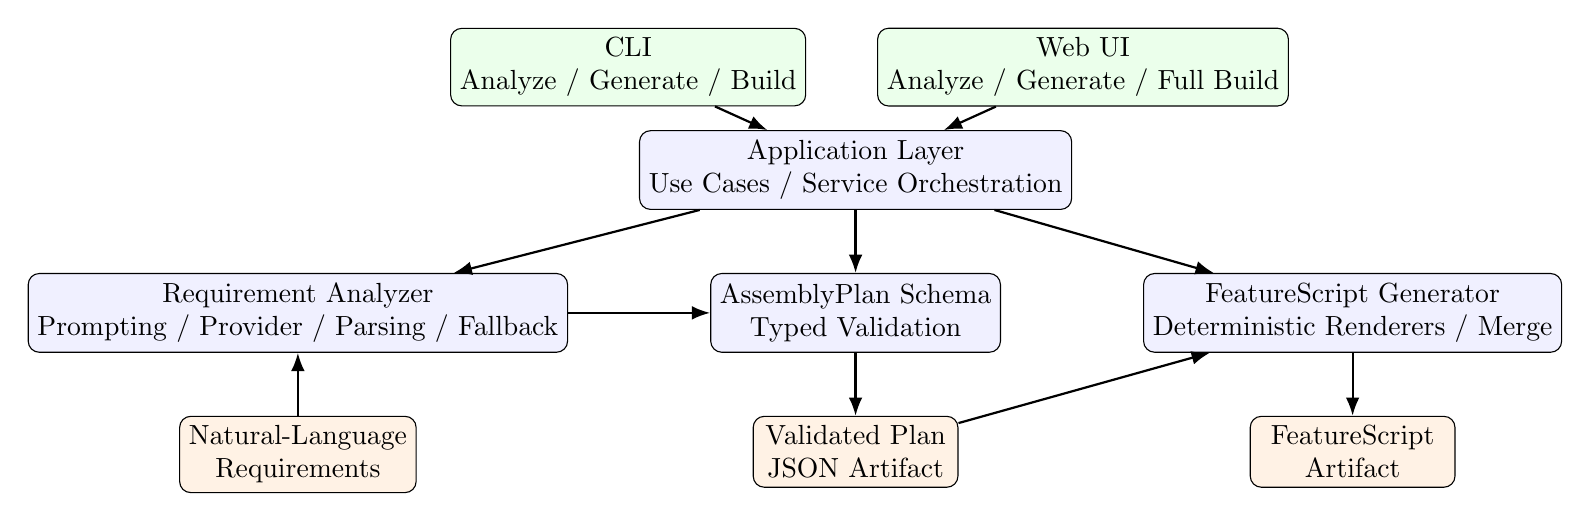
\begin{tikzpicture}[
  node distance=0.8cm and 0.9cm,
  >=Latex,
  box/.style={draw, rounded corners, align=center, minimum width=3.0cm, minimum height=1.0cm, fill=blue!6},
  io/.style={draw, rounded corners, align=center, minimum width=2.6cm, minimum height=0.9cm, fill=green!8},
  store/.style={draw, rounded corners, align=center, minimum width=2.6cm, minimum height=0.9cm, fill=orange!10},
  line/.style={->, thick}
]

\node[io] (cli) {CLI\\Analyze / Generate / Build};
\node[io, right=of cli] (web) {Web UI\\Analyze / Generate / Full Build};
\node[box, below=of $(cli)!0.5!(web)$] (app) {Application Layer\\Use Cases / Service Orchestration};
\node[box, below left=of app] (analysis) {Requirement Analyzer\\Prompting / Provider / Parsing / Fallback};
\node[box, below=of app] (schema) {AssemblyPlan Schema\\Typed Validation};
\node[box, below right=of app] (gen) {FeatureScript Generator\\Deterministic Renderers / Merge};
\node[store, below=of analysis] (req) {Natural-Language\\Requirements};
\node[store, below=of schema] (plan) {Validated Plan\\JSON Artifact};
\node[store, below=of gen] (fs) {FeatureScript\\Artifact};

\draw[line] (cli) -- (app);
\draw[line] (web) -- (app);
\draw[line] (app) -- (analysis);
\draw[line] (app) -- (schema);
\draw[line] (app) -- (gen);
\draw[line] (req) -- (analysis);
\draw[line] (analysis) -- (schema);
\draw[line] (schema) -- (plan);
\draw[line] (plan) -- (gen);
\draw[line] (gen) -- (fs);

\end{tikzpicture}
}
  \caption{系统总体架构。系统围绕“需求分析、Plan 校验、确定性脚本生成”三层核心能力展开，并同时服务于 CLI 与 Web UI 两类入口。}
  \label{fig:architecture}
\end{figure}

\subsection{系统架构设计}

从代码结构来看，系统主要由 \texttt{analysis}、\texttt{models}、\texttt{generation}、\texttt{application}、\texttt{io}、\texttt{webui} 和 \texttt{cli} 七类模块组成，分别负责模型分析、Schema 定义、模板生成、流程编排、文件读写、页面服务和命令入口。该分层方式使 CLI 与 Web UI 不直接实现业务逻辑，而是通过应用层与服务层复用同一套分析和生成流程。

\subsection{数据结构设计}

系统的核心中间表示为 \texttt{AssemblyPlan}。该结构至少包含以下字段：
\begin{enumerate}[leftmargin=2em]
  \item \texttt{assembly\_name}：装配体标识；
  \item \texttt{description}：装配描述；
  \item \texttt{global\_params}：全局尺寸信息和坐标原点描述；
  \item \texttt{parts}：零件列表；
  \item \texttt{assembly\_relations}：零件之间的装配关系。
\end{enumerate}

其中每个零件需要描述 \texttt{id}、\texttt{name}、\texttt{shape}、\texttt{material\_hint}、\texttt{params}、\texttt{position} 和 \texttt{description}。当前系统仅支持五种基础形状，这一限制是为了确保模板映射明确、参数集合稳定。

\subsection{关键流程设计}

\subsubsection{Analyze 流程}

Analyze 流程用于将需求文本转换为 Plan。应用层首先读取需求文本，然后调用 \texttt{RequirementAnalyzer}。分析器会使用预设提示词向大模型发起请求，获取流式返回内容，再尝试解析为 JSON 对象，并通过模型层进行严格校验。若模型调用失败或返回异常，而当前输入又匹配仓库内置样例，则系统会启用示例兜底逻辑，保证演示链路可运行。

\subsubsection{Generate 流程}

Generate 流程面向已有 Plan 文件。系统读取并校验 Plan 后，遍历全部零件，根据零件形状选择对应渲染器生成 FeatureScript 代码片段。所有片段最终由合并模块封装为标准 FeatureScript 文件。

\subsubsection{Build 流程}

Build 是全流程入口。它既可以接收自然语言需求，也可以在给定 \texttt{--plan} 时跳过分析阶段，直接进入生成。最终系统会输出 Plan 文件和 FeatureScript 文件，适合用于教学演示和批量脚本化使用。

\subsection{交互设计}

\subsubsection{CLI 设计}

CLI 是系统的主入口，支持多子命令。其优势在于可脚本化、便于集成、适合开发者调试和自动化验证。命令参数允许用户指定输入文本、输入文件、输出目录、分析模型、API Key 等运行时配置。

\subsubsection{Web UI 设计}

Web UI 面向演示场景，采用本地 HTTP 服务加静态前端页面方式实现。页面支持需求输入、样例填充、Plan JSON 编辑、FeatureScript 预览、结果摘要展示以及日志回显。由于 Web UI 直接复用后端 \texttt{WebUIService} 的能力，因此其分析与生成结果与 CLI 保持一致。

\section{系统详细实现}

\subsection{需求分析模块实现}

需求分析模块位于 \texttt{src/fs\_builder/analysis} 目录下，主要由请求适配、返回解析、异常处理和兜底方案组成。

系统预置了分析提示词，明确要求模型输出唯一合法 JSON，禁止返回说明文字与 Markdown 包裹。提示词中还定义了五种允许的零件形状、各形状必需的参数字段以及装配关系类型。这种约束设计的目的在于缩小模型输出空间，并降低后处理复杂度。

在请求实现上，系统支持通过 OpenAI 兼容接口发起流式分析请求，并允许配置模型名、超时时间和最大 token 数。为提高鲁棒性，模块设计了多轮 token 尝试和空内容重试机制；当接口返回空响应时，系统会降低最大 token 再次尝试，而不是立即失败。

为保证本地展示体验，分析模块还实现了一个仅针对仓库内置样例的 fallback 机制。以冷拉延模具示例为例，即使未配置 API Key，系统仍可基于文本中的关键尺寸规则生成一个演示用 Plan。这一机制并不面向通用需求，而是服务于课程答辩和项目展示。

\subsection{Plan 校验模块实现}

Plan 校验是整套系统可靠性的关键。系统使用统一的强类型模型完成命名约束、形状约束、参数约束、数值约束和关系约束。例如，\texttt{flange} 要求法兰直径必须大于轴直径，\texttt{tapered\_cylinder} 必须同时提供顶部直径、底部直径和高度。通过这些规则，系统能够在 FeatureScript 生成前拦截大多数结构性错误。

\subsection{确定性脚本生成模块实现}

与许多直接让模型生成代码的方案不同，本文系统的生成阶段完全采用确定性模板。\texttt{generation/renderers.py} 中为每种零件形状实现了专用渲染器：
\begin{enumerate}[leftmargin=2em]
  \item \texttt{box} 映射为立方体特征；
  \item \texttt{cylinder} 映射为圆柱体特征；
  \item \texttt{hollow\_cylinder} 通过外圆柱减内圆柱实现；
  \item \texttt{tapered\_cylinder} 通过锥台几何实现；
  \item \texttt{flange} 通过法兰体与轴体的并集实现。
\end{enumerate}

每个渲染器只关心本类零件的参数提取与几何表达。由于这些逻辑完全由程序控制，因此输出结果具有较高稳定性。生成模块还设计了错误隔离机制：当某个零件生成失败时，系统会记录失败信息而不是立即中断整体输出，最终在结果脚本中以内联注释形式保留错误原因。

\subsection{脚本合并与输出实现}

在局部零件代码片段生成后，系统会统一组装为标准 FeatureScript 文件。输出文件头包含生成时间、装配体名称和简要描述；主体部分则按零件顺序依次插入代码块。对成功零件，会保留可读的名称注释与实体命名；对失败零件，会输出错误提示注释。

这种设计的优点在于，最终产物既是程序生成结果，也保留人工可读和可修改性。

\subsection{CLI 与应用层实现}

应用层 \texttt{use\_cases.py} 将系统能力封装为四类核心用例：\texttt{analyze\_command}、\texttt{validate\_plan\_command}、\texttt{generate\_command} 和 \texttt{build\_command}。CLI 层仅负责参数解析与错误输出，不直接处理业务逻辑，从而降低了命令入口与系统核心逻辑的耦合程度。

这种设计使自动化测试可以直接针对应用层调用，而不必全部通过子进程方式驱动 CLI，同时也便于 Web UI 复用同类能力。

\subsection{Web UI 实现}

系统 Web UI 采用 Python 标准库中的 \texttt{ThreadingHTTPServer} 提供本地 HTTP 服务，前端部分由静态 HTML、CSS 和 JavaScript 构成。用户可以选择 Analyze、Generate 或 Full Build 三种运行模式，并直接查看结果摘要。

相较于额外引入复杂 Web 框架，这种实现方式更轻量，便于本地答辩演示和部署。Web UI 通过 \texttt{WebUIService} 直接复用后端分析与生成能力，从而保证界面与命令行结果一致。

\section{系统测试与结果分析}

\subsection{测试目标与测试环境}

系统测试重点围绕以下问题展开：
\begin{enumerate}[leftmargin=2em]
  \item 中间表示是否能稳定校验；
  \item 分析、生成、合并流程是否可正常运行；
  \item CLI 与 Web UI 是否能够正确调用核心能力；
  \item 对典型样例，系统是否能给出完整输出；
  \item 异常输入是否会被合理拦截。
\end{enumerate}

测试环境基于项目自带 Python 虚拟环境执行，核心验证命令包括自动化测试与样例构建命令。由于当前仓库尚未接入 Onshape 在线编译回读闭环，因此本文测试重点放在本地逻辑正确性、脚本生成完整性和接口调用一致性上。

\subsection{自动化测试结果}

在项目当前版本下，执行自动化测试命令后，共有 50 项测试全部通过，执行时间约为 2.37 秒。进一步统计覆盖率后，项目总代码覆盖率达到 82\%。主要覆盖对象包括 \texttt{models}、\texttt{analysis}、\texttt{generation}、\texttt{application}、\texttt{cli}、\texttt{io} 和 \texttt{webui} 等模块。

\begin{table}[H]
  \centering
  \caption{系统核心验证指标}
  \label{tab:main-metrics}
  \begin{tabular}{p{5.2cm}cc}
    \toprule
    指标 & 数值 & 说明 \\
    \midrule
    自动化测试通过数 & 50 & 本地 \texttt{pytest} 结果 \\
    代码覆盖率 & 82\% & \texttt{pytest --cov} 统计结果 \\
    支持零件形状数 & 5 & 受限任务域设置 \\
    冷拉延模具样例成功率 & 5/5 & 全部零件成功生成 \\
    \bottomrule
  \end{tabular}
\end{table}

覆盖率明细显示，覆盖相对较低的部分主要是 \texttt{webui/server.py} 的 HTTP 处理细节与部分兼容层入口文件。这说明系统已经对核心业务逻辑做了较充分验证，但在端到端浏览器交互方面仍有继续补充测试的空间。

\begin{figure}[H]
  \centering
  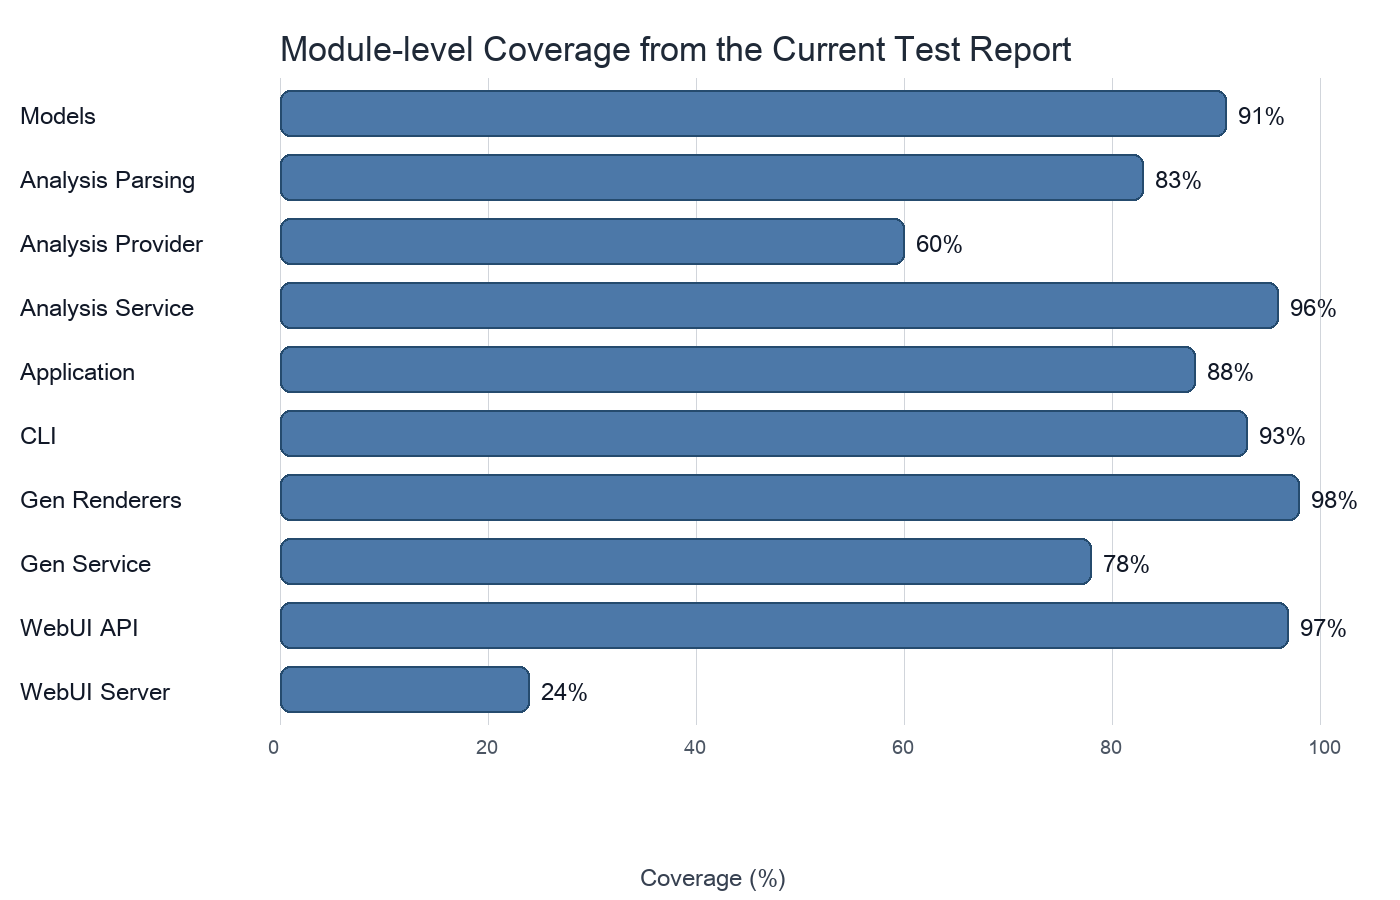
\includegraphics[width=0.94\linewidth]{figures/coverage_chart_python.png}
  \caption{基于真实覆盖率报告绘制的模块级覆盖率对比图。该图由 Python 脚本自动生成，并作为评测结果图直接纳入正文。}
  \label{fig:coverage-chart}
\end{figure}

\subsection{典型样例验证}

为了验证系统完整链路，本文选取仓库内置的“冷拉延模具”需求文本作为典型样例进行构建测试。该样例描述了上模座、下模座、凹模、压边圈和凸模五个主件，并给出了关键尺寸约束。执行构建命令后，系统成功输出一个结构化 Plan 文件、一个完整 FeatureScript 文件，并实现 5/5 零件全部生成成功。

从生成结果可见，系统将自然语言需求转换为一个包含 5 个零件和 4 条装配关系的装配 Plan。其中，下模座和上模座被识别为 \texttt{box}，凸模被识别为 \texttt{cylinder}，凹模和压边圈被识别为 \texttt{hollow\_cylinder}。在 FeatureScript 输出中，系统进一步将这些零件映射为立方体、圆柱体和布尔减运算等稳定几何操作。

该样例验证说明，在受限任务域内，系统不仅能理解结构性需求，还能形成符合模板约束的参数化输出。

\subsection{结果分析}

从测试与样例结果看，本文系统具有以下优点：一是结构清晰且工程闭环完整；二是中间表示设计有效，能够通过 Plan 约束收缩自然语言带来的不确定性；三是演示友好，CLI 与 Web UI 复用同一套服务逻辑；四是错误处理较为明确，需求缺失、Plan 非法或零件生成失败时都能给出可理解反馈。

但系统也存在明显局限：
\begin{enumerate}[leftmargin=2em]
  \item 目前仅支持五种基础零件形状，无法覆盖更复杂的孔、圆角、倒角和复杂装配约束；
  \item 尚未与 Onshape 编译结果建立自动闭环，因而当前验证重点仍是“脚本生成正确性”，而非“云端 CAD 执行正确性”；
  \item 当前缺少真实用户实验和大规模需求集合测试，无法从统计意义上评价系统在开放域需求下的鲁棒性；
  \item 分析阶段仍依赖外部大模型接口，在没有 API Key 的一般场景下无法完成通用需求分析，当前 fallback 仅服务于内置演示样例。
\end{enumerate}

\section{总结与展望}

本文围绕“面向简单机械结构建模的自然语言驱动参数化 CAD 生成系统”这一主题，设计并实现了 \texttt{fs-builder} 项目。系统采用大语言模型负责需求理解、强类型 Plan 负责中间约束、确定性模板负责最终脚本生成的架构路线，在自然语言灵活性与 CAD 脚本稳定性之间取得了较好的工程平衡。项目自动化测试全部通过，典型冷拉延模具样例实现了 5 个零件的完整脚本生成，说明系统在限定任务域内具有可行性和实用价值。

本课题的核心价值并不在于实现一个开放域 CAD 智能体，而在于提出并验证了一种适合本科毕业设计场景的工程方法：让大模型只做其擅长的语义理解，让程序化中间层承担约束收缩，让确定性模板负责最终产物落地。

后续工作可从以下几个方向展开：
\begin{enumerate}[leftmargin=2em]
  \item 扩展几何能力，增加孔、沉头孔、倒角、圆角、阵列和螺纹孔等常见特征；
  \item 引入装配约束求解，使系统不仅能表达零件叠放关系，还能进一步处理同轴、平行和间隙等约束；
  \item 接入 Onshape 编译与回读闭环，自动检测 FeatureScript 是否成功编译，并将编译反馈用于纠错；
  \item 增强交互式修订能力，在 Web UI 中加入参数修改、差异对比和增量重生成功能；
  \item 建立评测集，从成功率、字段完整率和脚本有效率等指标系统评估工具质量。
\end{enumerate}

综上，本文完成了一个具备完整闭环、结构清晰、可验证、可展示的毕业设计系统。该系统虽然能力范围有限，但在“自然语言输入 + 受控中间层 + 参数化脚本输出”这一方向上提供了一个具有实践价值的实现样例。

\begin{thebibliography}{99}

\bibitem{vaswani2017attention}
Vaswani, A., Shazeer, N., Parmar, N., Uszkoreit, J., Jones, L., Gomez, A. N., Kaiser, {\L}., \& Polosukhin, I. (2017). Attention is all you need. \textit{arXiv}. \url{https://arxiv.org/abs/1706.03762}

\bibitem{openai2023gpt4}
OpenAI. (2023). GPT-4 technical report. \textit{arXiv}. \url{https://arxiv.org/abs/2303.08774}

\bibitem{seff2020sketchgraphs}
Seff, A., Ovadia, Y., Zhou, W., \& Adams, R. P. (2020). SketchGraphs: A large-scale dataset for modeling relational geometry in computer-aided design. \textit{arXiv}. \url{https://arxiv.org/abs/2007.08506}

\bibitem{wu2021deepcad}
Wu, R., Xiao, C., \& Zheng, C. (2021). DeepCAD: A deep generative network for computer-aided design models. \textit{arXiv}. \url{https://arxiv.org/abs/2105.09492}

\bibitem{khan2024text2cad}
Khan, M. S., Sinha, S., Sheikh, T. U., Stricker, D., Ali, S. A., \& Afzal, M. Z. (2024). Text2CAD: Generating sequential CAD designs from beginner-to-expert level text prompts. In \textit{Advances in Neural Information Processing Systems} (Vol. 37). \url{https://proceedings.neurips.cc/paper_files/paper/2024/hash/0e5b96f97c1813bb75f6c28532c2ecc7-Abstract-Conference.html}

\bibitem{onshape_fsdoc}
Onshape. (n.d.). FeatureScript documentation. \url{https://cad.onshape.com/FsDoc/index.html}

\bibitem{onshape_featurescript}
Onshape. (n.d.). Custom features. \url{https://www.onshape.com/featurescript}

\end{thebibliography}


\appendix
\section{Mermaid 流程图源文件说明}
Mermaid 流程图源文件位于 \texttt{figures/pipeline\_flow.mmd}，用于在文档工具链或答辩展示中复用系统流程图。考虑到 Mermaid 并非标准 LaTeX 绘图库，本文正文采用 TikZ 图进行排版，Mermaid 源文件作为附加可视化资产随论文一并提供。

\end{document}
